%!TEX root = ../crimson_throne_book_main.tex
% 2015-01-03
\section{1 Erastus 4708}

The companions get their horses ready for the trip to {\itshape Lost End} and pick up their charter at Citadel Volshyenek. The Field Marshal also hands them a reward for closing Lavender's Luxury two days ago: a hefty pouch with 1,000 gold sails and some of the swindlers' equipment, a magical greatsword, mithral breastplate and cloak, which all go the Balian, and a  {\itshape ring of protection} for Quint. Then the heroes leave the city. The farmland makes way for a rougher terrain after a couple of hours as the road bends off to the west and crawls between the western stretches of the Mindspin Mountains that line the southern horizon and the cliffs alongside the Bay of Korvosa somewhere to the north. The sole pathway here sees infrequent passage, as only the Hellknights from Citadel Vraid travel it from time to time on their heavy warhorses, but the heroes do not encounter any of these blind enforcers of the law today. When darkness sets, they make camp and pass a restful night.\\

\section{2 Erastus 4708}

After a couple of hours Balian spots an overgrown path that veers off the main road to the northwest. Travel becomes slower now, as the horses have to walk through the high grass and weeds. It definitely looks as if no one has come this way for a long time.\\

It is almost noon when the companions pick up the muffled murmur of pain from behind the bushes. They dismount and check out the source of the noise, discovering a large wounded bear that has a bear trap around its paw. It has been pulling at the iron teeth to try and get free, but its efforts have only caused it further injury. The animal roars viciously when the adventurers approach, giving them pause. Suddenly the growls of the injured colossus are drowned by barking dogs, who are closing in fast. A few breaths later six hunting hounds burst out of the foliage and attack both the bear and the companions. Despite their fervor the dogs cannot penetrate the companions' defenses and soon start to fall prey to their weapons.\\

"You hurts my dogs! Rukus Graul kill you for that, he will!" The master of the hounds arrives in the wake of his pack. It is an\hyperref[fig:Rukus-Graul-504564975]{ ugly humanoid with a wide mouth and a huge misshapen finger which dangles like a hook from his right hand } . Quint recognizes the creature as ogrekin, like the grotesque cabbage-headed hulk the heroes encountered in the derro warrens, an unnatural mix of humans and ogres. The lumbering hunter wields a sharp spear, but fails to hit Balian. At the same time the hounds finish off the bear and now hurl themselves on the companions. The heroes pick off the mongrels one at a time without suffering a single bite. The unfortunate half-ogre is equally unsuccessful and never scores a hit with his spear. Sjo barks at him to surrender, but he refuses. "You kill my dogs, I kill yours!" he grunts as he plunges his pike in Spyder. "Rukus not surrender, ever!" he shouts as the companions bear down on him from all sides. The next moment his dead body drops to the ground. That is how the heroes of Korvosa deal with stupid, overconfident brutes. \\

\begin{figure}[h]
	\centering
	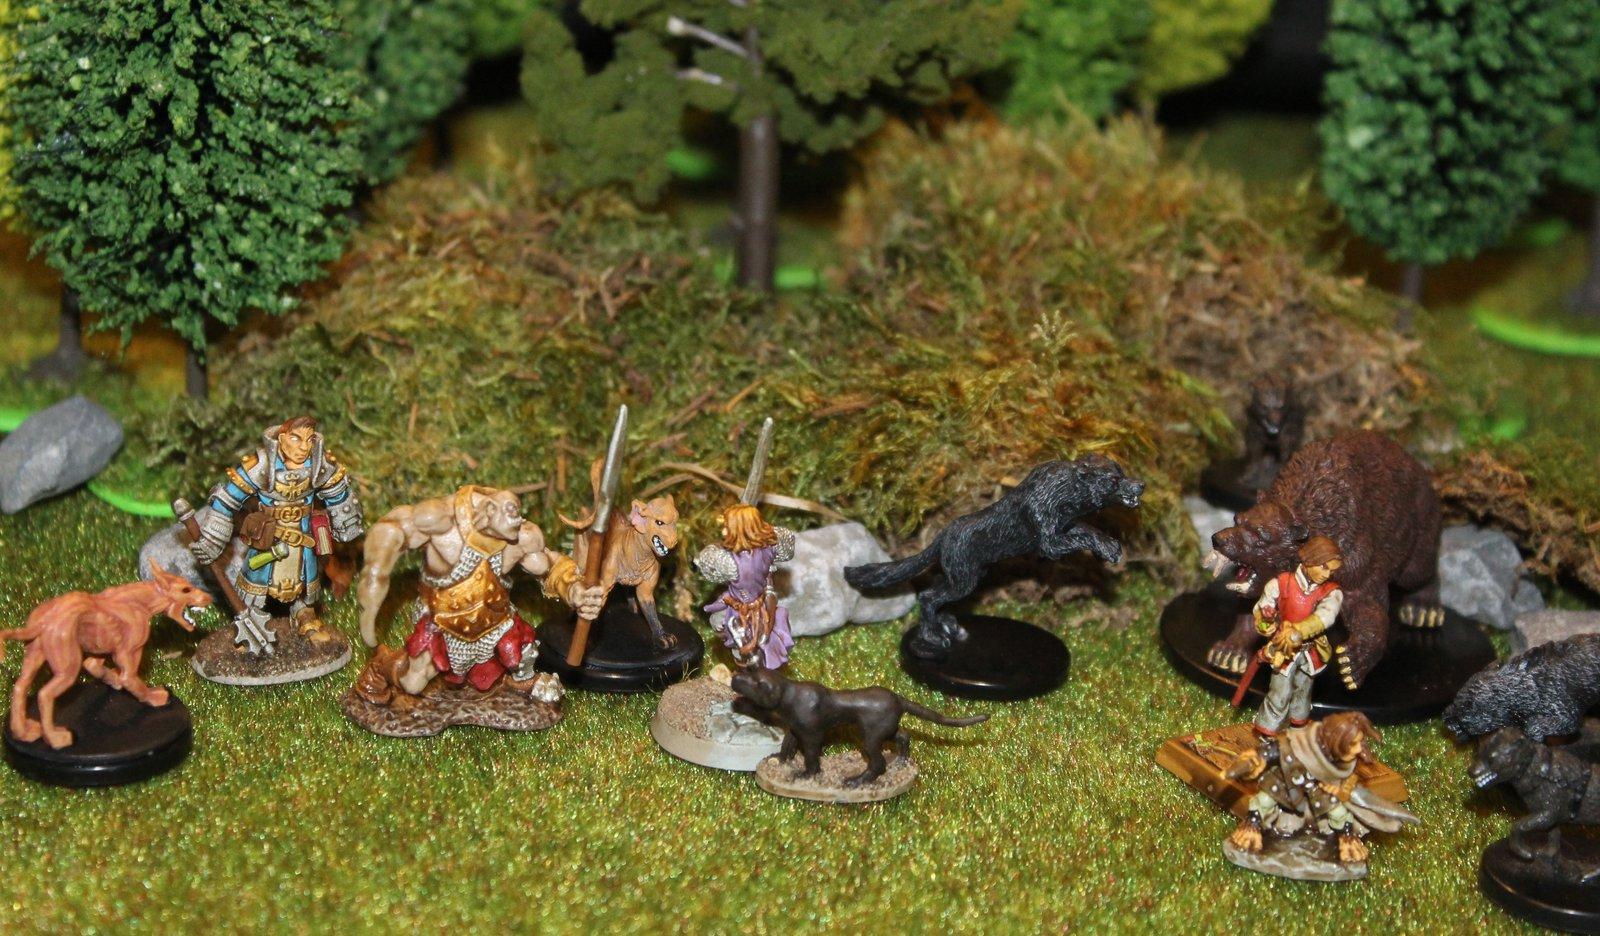
\includegraphics[width=0.39\textwidth]{images/Rukus-Graul-504564975.jpg}
	\caption{Rukus Graul}
	\label{fig:Rukus-Graul-504564975}
\end{figure}

Using {\itshape detect magic} Sjo is pleasantly surprised to learn that this primitive creature was wearing a valuable girdle around his waist, a  {\itshape belt of giant strength} , which the Shoanti healer gladly straps around his own hips. 